\chapter{Camera Pose Verification}

In the chapter, datasets, their transformations, and experiments performed upon them with
the introduced methods' implementations are all presented. We use the generalized InLoc
pipeline with a modified pose verification step. The synthesized image leveraged for
pixel-wise computation of similarity with the given query image is swapped with views
generated by renderers presented in the preceding chapter, depicting the scene's point
cloud from estimated query positions. Apart from how the synthesized image is generated,
the rest of the verification process is then performed according to the original article,
using namely RootSIFT descriptors.\\

While discussing concrete details of datasets' definitions and algorithms' inputs, more
technical aspects are taken into account---among them, of utmost importance are
conventions used by coordinate systems in which points of explicit scene representations
are expressed/expected to be and by matrices related to cameras taking database images.
These pose a crucial difference between what a dataset provides, or localization pipeline
expects and must be addressed by implementation to obtain valid localization results.

\begin{figure}
    \centering
    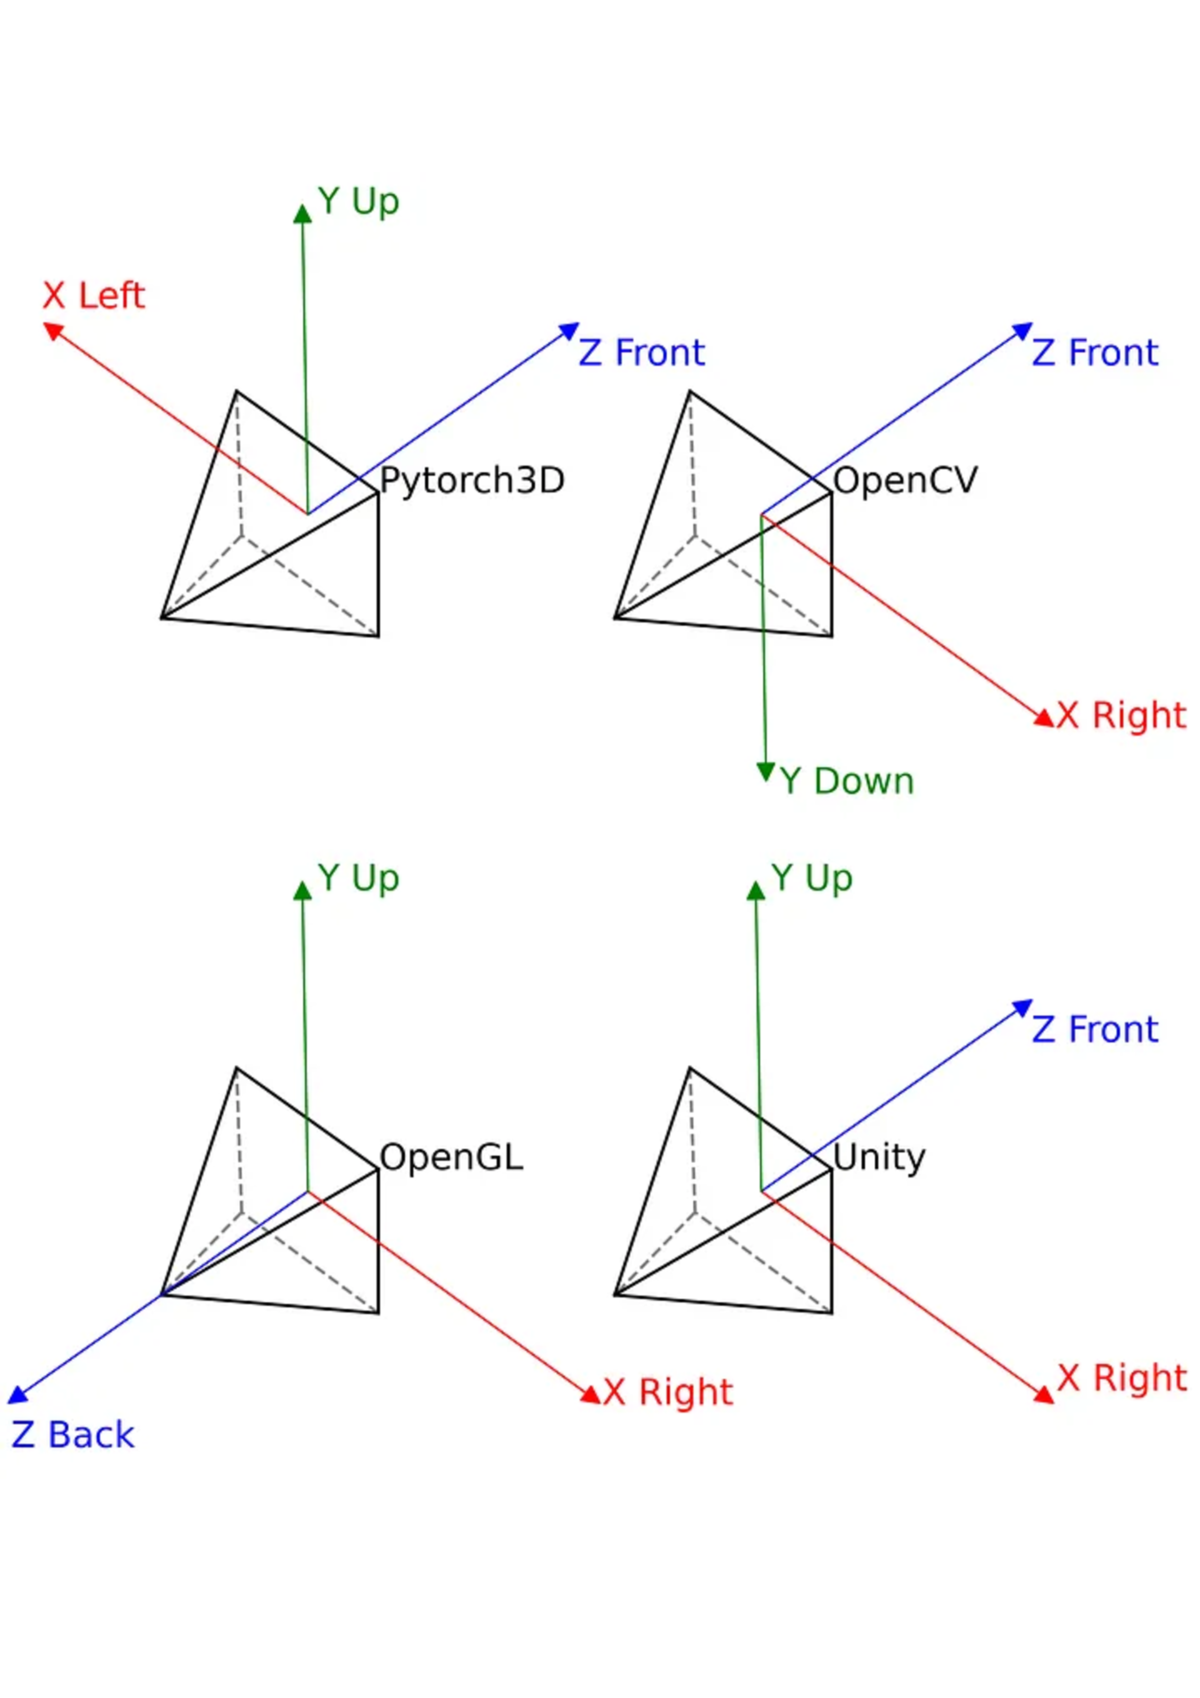
\includegraphics[width=.7\textwidth]{../graphics/cs_conventions.pdf}
    \caption{Examples of various camera / coordinate frame conventions used by
    common programmatic tools in fields dealing with computer graphics.
    Taken from~\url{https://medium.com/check-visit-computer-vision/converting-camera-poses-from-opencv-to-opengl-can-be-easy-27ff6c413bdb}.}\label{fig:cs_conventions}
\end{figure}

Coordinate system conventions address the decision of assigning positive directions,
labels, and meanings in the human sense (up, right, forward) to the orthogonal frame of a
3D space, because without that an oriented triplet representing a point is meaningless.
These conventions can be arbitrary depending on whether they come from computer vision,
rendering, or another field. Examples of such conventions, linked to standard computer
graphics libraries/tools that use/expect them, can be found in~\cref{fig:cs_conventions}.
In this thesis, computer vision and rendering conventions are used. In the
figure~\cref{fig:cs_conventions}, these are found alongside OpenCV and OpenGL labels,
respectively. Even though both are right-handed, they understand x, y, and z point
components differently.  In rendering, the positive x-axis points to the right, the
positive y-axis up, and the positive z-axis towards a viewer looking at the coordinate
system frame. In computer vision, the positive x-axis points to the right, the positive
y-axis to the bottom, and the z-axis away from the same viewer as before. Transformation
matrices operating over both notations are thus related by inverting the y and z axes
columns. As an example, since a camera in rendering is typically placed along z-xis,
failing to take this relation into account when displaying a 3D model defined in computer
vision notation in a visualization tool that uses rendering notation results in rendering
half-space \uv{away} from the model. For instance, in the case of other notations used by
a produced model, a rendered view can be somewhat unexpectedly rotated.

Matrix conventions in the context of the thesis are related to terms coming from the
graphics pipeline---\emph{world space} and \emph{view space}. In the case of datasets
described below, world space is a space of the whole scene representation with the origin
and orientation of the coordinate frame chosen arbitrarily in relation to the scene.  The
randomness in the coordinate frame placement is especially true in the case of
SfM-generated scene models, where the algorithm decides these parameters.  When preparing
a model manually, e.g., in the game industry, the frame is typically artificially placed
meaningfully concerning the model produced, e.g., along the outer edges of a cube model.
View space is a space of a camera looking at a portion of the scene---origin is the center
of the camera with the coordinate frame oriented in a specific way alongside the optical
axis of the camera depending on the exact graphics pipeline/tool used.
Visualisation~\cref{fig:cs_conventions} can be used here as well---the square pyramids
depict view frustums of virtual cameras, with the z-axes being their optical axes.

Provided both spaces are same-handed, the matrix inverse relates transformations between
them. In homogeneous coordinates, both transformations are represented by $4\times4$
matrices, and the implementation must correctly distinguish between the actual meaning of
these 16~real numbers, including how the matrix is stored on the disk. We refer to them as
the \emph{view matrix} transforming from world to view space and \emph{camera pose}
representing the opposite, inverse transformation.

\section{Datasets}

Several image collections were used for measuring localization performance, both indoors
and outdoors. To ensure continuity and comparability with previous works of~\citet{InLoc,
Bastien}, we utilize the open-source InLoc Dataset presented in the original Inloc
paper~\citep{InLoc}. Another closed-source, indoor dataset is a 3D scanner-generated
digital twin of a SIEMENS manufacturing facility that is targeted by several use cases of
the Industry \& Construction 4.0 Solutions project called ARTwin, financially supported by
the European Union's Horizon 2020 research and innovation program. Finally, an outdoor
dataset is covered by the inclusion of the open-source Phototourism dataset from the Image
Matching Challenge
2021\footnotei{.}{\url{https://www.cs.ubc.ca/research/image-matching-challenge/2021}}

\subsection{InLoc Dataset}

The dataset consists of a database of Faro 3D scanner-generated RGBD scans that are
geometrically registered to the floor plan of two buildings of Washington University in
St. Louis. The test set is a composition of RGB photos taken by a hand-held device (an
iPhone).

277 RGBD panoramic images have ground truth poses in the global coordinate system spanning
across the floor plan. Each RGBD panoramic scan is a point cloud (\emph{scan}) having
roughly 40~million colored points. The final dataset is generated by obtaining
36~perspective RGBD images from each panorama by extracting standard perspective views
($60^{\circ}$~FoV) with a sampling stride of $30^{\circ}$ in yaw and $\pm30^{\circ}$ in
pitch directions, resulting in cca 10~thousand perspective images in total, examples are
in~\cref{fig:inloc_dataset}. This dataset contains all troublesome elements for indoor
localization, namely repetitive patterns (such as stairs and pillars), global and local
similarities (doors, windows), furniture changing positions in the test set, people moving
across the scene, and textureless, highly symmetric areas (walls, floors, corridors,
classrooms, open spaces).

The original query set consists of 356~photos taken by an iPhone~7 at various lighting
conditions within a day, capturing a variety of occluders and layouts (people, furniture),
also covering only a subset of the floor plan data, with the rest playing the role of
confuser at search time. Ground truth poses for the test set are not publicly accessible,
and evaluation can be done only indirectly via submission to the Visual
Localization\footnote{\url{https://www.visuallocalization.net}} page.

The structure of the dataset's database folder is as follows---\verb|scans/<FLOOR>|
folders, where \verb|FLOOR| is one of DUC1, DUC2, CSE3, CSE4, and CSE5, representing five
floors of the two mentioned buildings (CSE, DUC), contain files named
\verb|<NAME_WITH_SCAN_NUMBER>.ptx.mat| storing RGB and XYZ information of scanned points
in Matlab file format. Every floor has its specific number of scans, uniquely numbered
within a building. Final dataset's perspective views are stored in folders
\verb|cutouts/<FLOOR>/<SCAN_NUMBER>| containing JPG perspective RGB images of size
$1600\times1200$ pixels and MAT files containing bundled RGB perspective image (RGBcut)
and the respective scan points (XYZcut). Files
\verb|alignments/<FLOOR>/transformations/<NAME_WITH_SCAN_NUMBER>.txt| contain $4\times4$
transformation matrices that convert 3D homogeneous points in original .ptx.mat files to
the global coordinate system of the floor plan.

The dataset's query folder contains one subfolder named \verb|iphone7| with the query set
of photos taken by the iPhone camera. Photos are stored as JPG files of size
$4032\times3024$ or $3024\times4032$ pixels, so both landscape and vertical acquisition
modes were used. As the database is landscape, for InLoc algorithm processing, all images
are made landscape, and the ones where the view was changed by rotation are remembered.
Notably, even though sharing the same aspect ratio with the database after such operation,
which InLoc localization pipeline can handle, resizing to the matching dimensions is also
used to speed up the localization performance.

\begin{figure}
    \centering
    \begin{subfigure}{.5\textwidth}
        \centering
        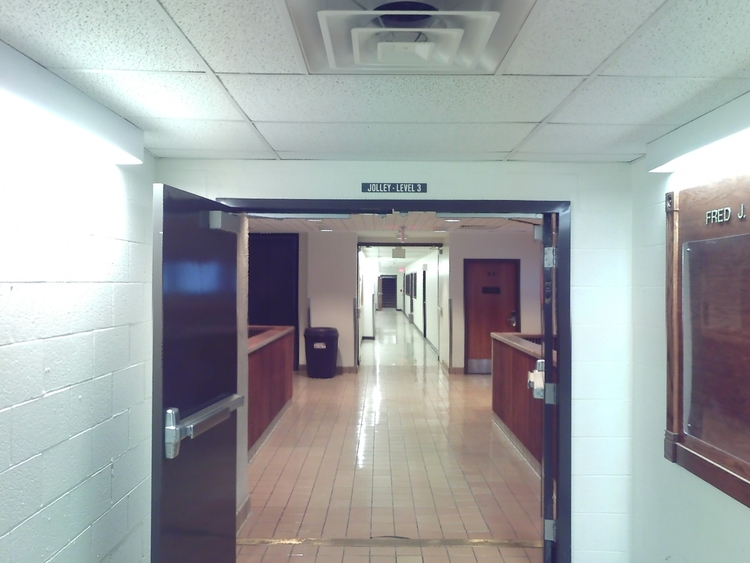
\includegraphics[width=.9\textwidth]{../graphics/cse_cutout_000_90_0.jpg}
    \end{subfigure}%
    \begin{subfigure}{.5\textwidth}
        \centering
        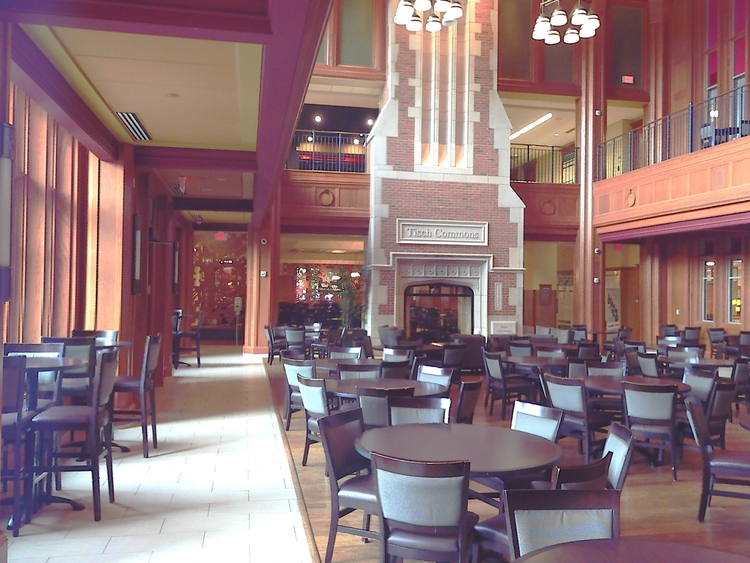
\includegraphics[width=.9\textwidth]{../graphics/DUC_cutout_003_0_0.jpg}
    \end{subfigure}
    \caption[Samples from InLoc dataset database images]{Samples from InLoc dataset database images.}\label{fig:inloc_dataset}
\end{figure}

\subsection{ARTwin Dataset}

The dataset consists of registered $360^{\circ}$ RGB panoramic images across two halls of
a SIEMENS manufacturing facility together with point clouds for both produced by merging
3D data from a NavVis 3D scanner.

Over the two halls, 29 and 53~panoramic images were obtained. The final dataset used in
this thesis contains roughly 4~thousand processed images and it is generated in accordance
with InLoc Dataset except for a difference in the necessity to remap
$360^{\circ}$~spherical panorama to 2D~surface again, examples are
in~\cref{fig:artwin_dataset}. Hall point clouds are not matched to a common coordinate
system as they overlap when displayed together, so for localization disambiguation one
hall is lifted along the z-axis.

The raw dataset contains all the intermediate files, photos and logs from the acquiring
process together with processed and merged results mentioned above. The structure of the
relevant processed data is \verb|proc/<HALL_ID>|, IDs of the halls are
\verb|2019-09-28_08.31.29| and \verb|2019-09-28_16.11.53|. Within each of these folders,
there is processed point cloud \verb|<HALL_ID>.ply| and \verb|pano| folder with JPG
panoramic scans alongside \verb|pano-poses.csv|. Poses are in the form of 3D scanner
position and orientation quaternion per panoramic scan.

\SaveVerb{hall53}|2019-09-28_16.11.53|
\SaveVerb{hall29}|2019-09-28_08.31.29|
\begin{figure}
	\centering
	\begin{subfigure}{.5\textwidth}
		\centering
		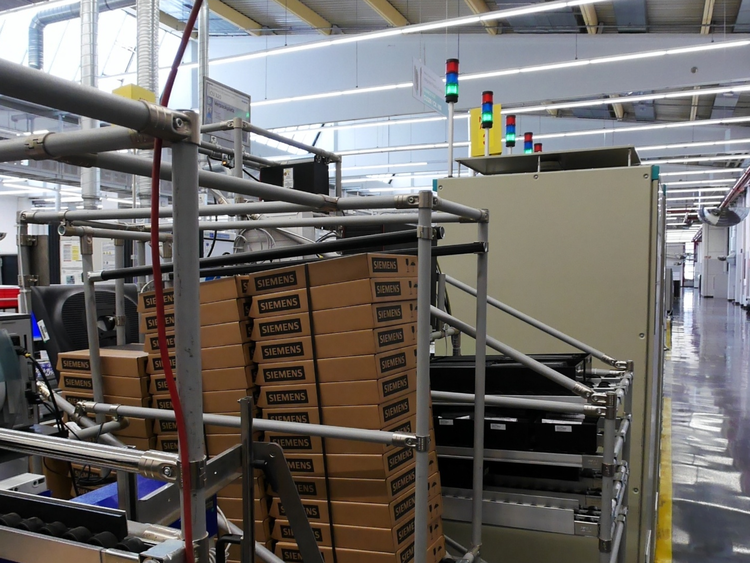
\includegraphics[width=.9\textwidth]{../graphics/2019-09-28_16.11.53_00000_x0_z90_reference.png}
	\end{subfigure}%
	\begin{subfigure}{.5\textwidth}
		\centering
		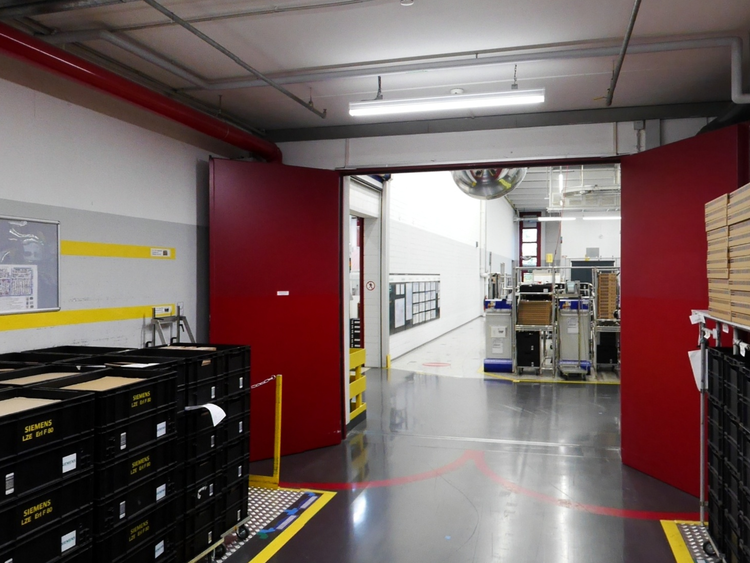
\includegraphics[width=.9\textwidth]{../graphics/2019-09-28_08.31.29_00000_x0_z60_reference.png}
	\end{subfigure}
	\caption[Sample flattened images from ARTwin dataset]{Sample
        flattened images from ARTwin dataset, on the left hall
        \protect\UseVerb{hall53} is presented, on the right
        \protect\UseVerb{hall29}.}\label{fig:artwin_dataset}
\end{figure}

\subsection{Phototourism Dataset}

The smallest datasets taken from the Image Matching Challenge (IMC) data, photo-tourism image
collections depicts several popular landmarks, collected from the Yahoo Flickr Creative
Commons 100M (YFCC) dataset. Namely, Hagia Sophia Interior, Pantheon Exterior, and Grand
Place Brussels collections were used. These datasets have around $1\,000$~photos each
coming, using the terminology from~\citet{NRIW}, \uv{from the wild} as they were taken by
many authors, at various distances and with sensor sizes varying considerably,
see~\cref{fig:imc_dataset}.

\begin{figure}
	\centering
	\begin{subfigure}{.5\textwidth}
		\centering
		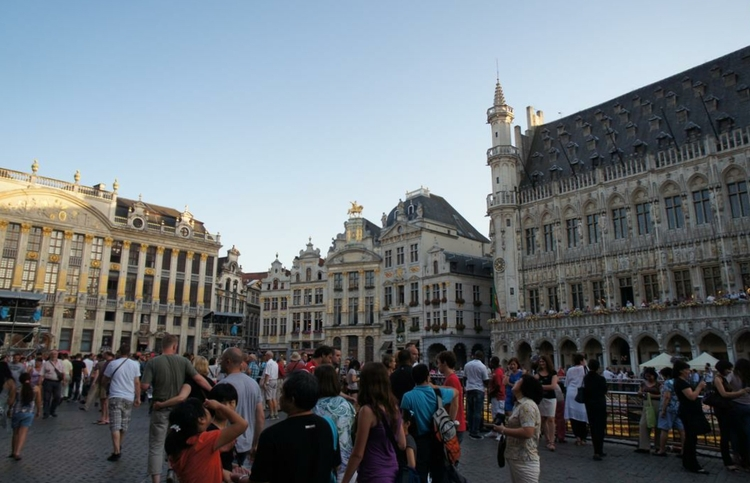
\includegraphics[width=.9\textwidth]{../graphics/grand_06498281_8296173847.jpg}
	\end{subfigure}%
	\begin{subfigure}{.5\textwidth}
		\centering
		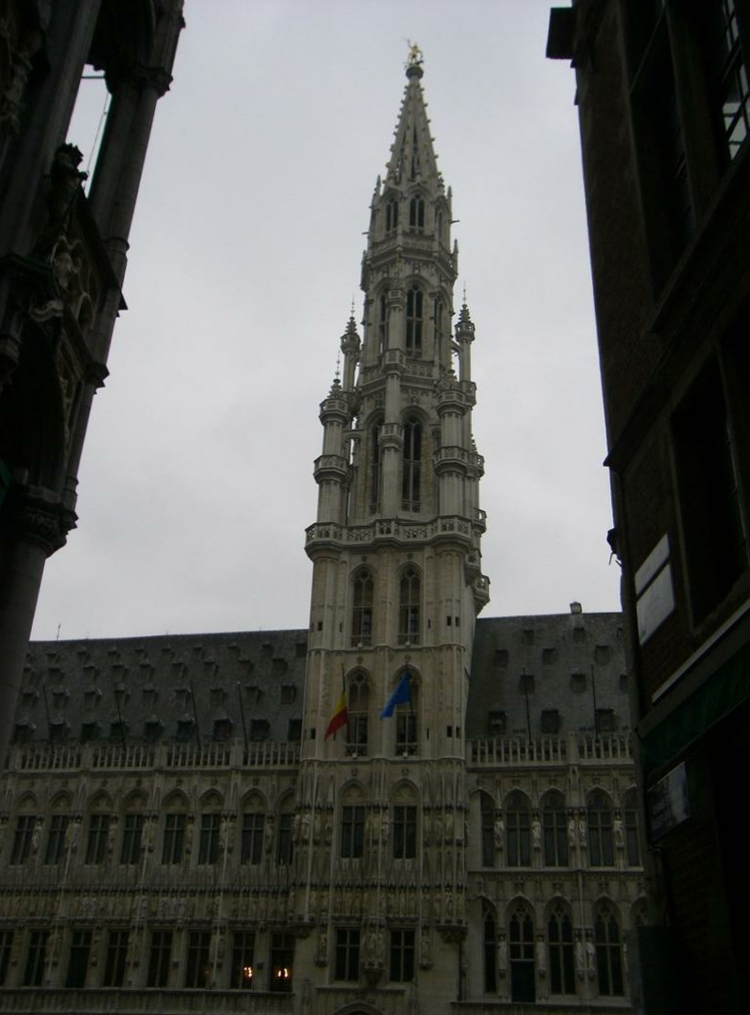
\includegraphics[width=.9\textwidth]{../graphics/grand_01352021_435013564.jpg}
	\end{subfigure}
	\begin{subfigure}{.5\textwidth}
		\centering
		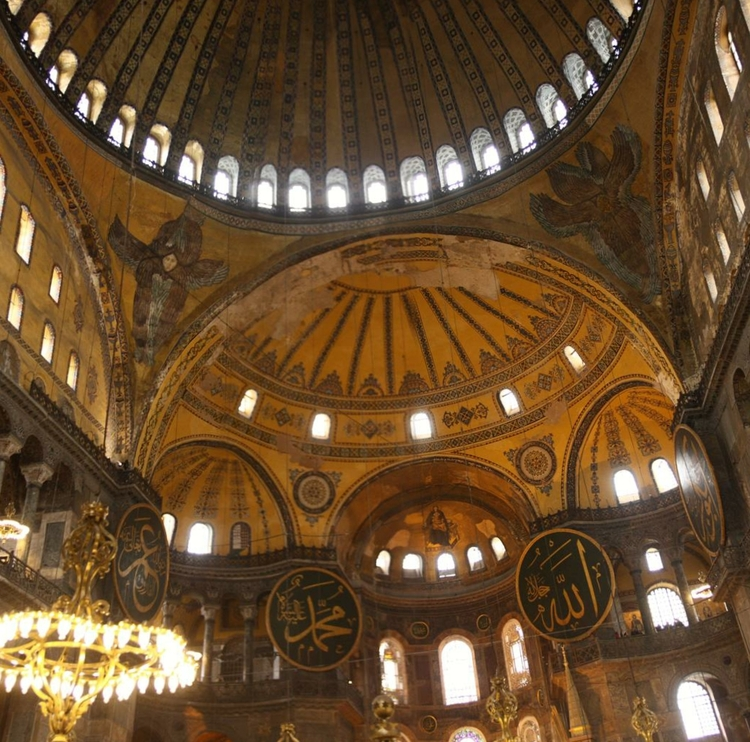
\includegraphics[width=.9\textwidth]{../graphics/hagia_04240457_5644708528.jpg}
	\end{subfigure}%
	\begin{subfigure}{.5\textwidth}
		\centering
		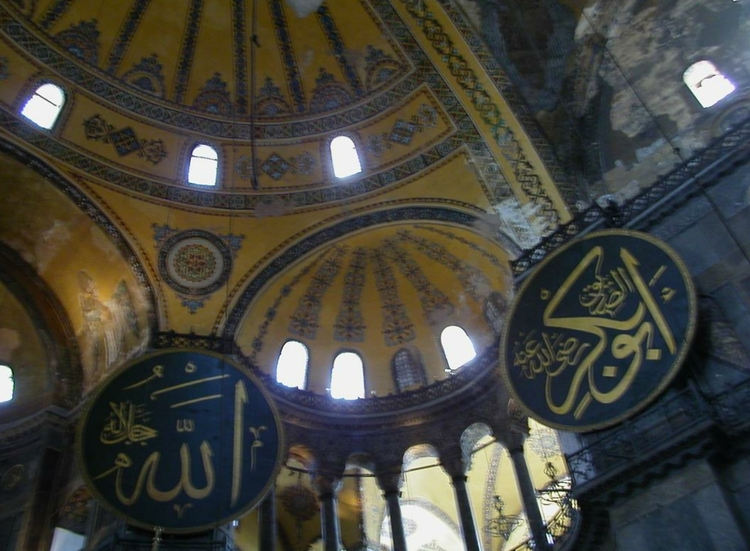
\includegraphics[width=.9\textwidth]{../graphics/hagia_01058134_62294335.jpg}
	\end{subfigure}
	\begin{subfigure}{.5\textwidth}
		\centering
		
\includegraphics[width=.9\textwidth]{../graphics/pantheon_00488011_10505838106.jpg}
	\end{subfigure}%
	\begin{subfigure}{.5\textwidth}
		\centering
		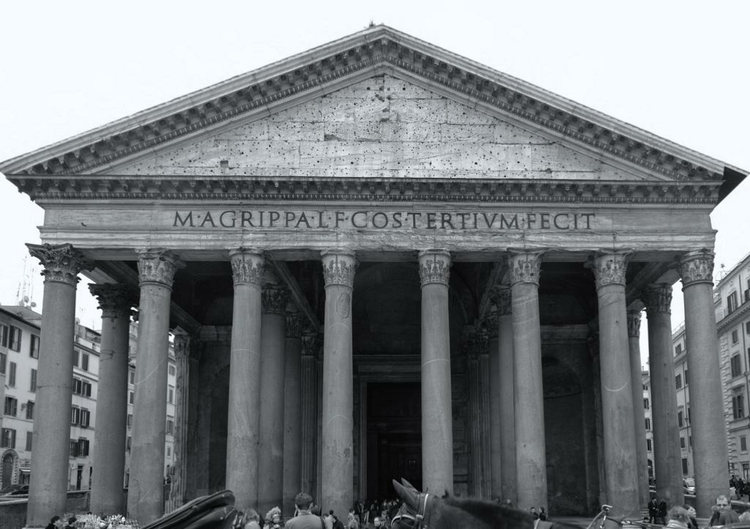
\includegraphics[width=.9\textwidth]{../graphics/pantheon_00927614_8536847775.jpg}
	\end{subfigure}
	\caption[Sample images from Phototourism dataset]{Sample images from
        Phototourism dataset taken \uv{from
        the wild}, stretching various aspect ratios, sizes, time of the day of the
        aquisition, and varying lighting conditions present in the data. In the top
        row there are images of Grand Place in Brussels, below of interior of Hagia
        Sophia Grand Mosque in Istanbul, and in the bottom of Pantheon in
        Rome.}\label{fig:imc_dataset}
\end{figure}

The dataset per given collection used in the thesis is built on top of raw images by
running COLMAP software. Structure of the COLMAP produced dataset is described in its
documentation\footnotei{.}{\url{https://colmap.github.io/format.html}} Shortly, there is
\verb|dense/sparse/cameras.bin| file with parameters of cameras capturing wild images
retrieved by SfM method implemented in COLMAP, \verb|dense/sparse/images.bin| file with
retrieved 3D positions and orientation quaternions of each image in a common coordinate
system of \verb|dense/fused.ply| point cloud. This point cloud is generated by SfM from
implicit scene representation contrary to the previously mentioned datasets that represent
a 3D scanner-generated approach.\\

Putting everything together---all scene point clouds for all datasets explored in the
thesis are placed in the right-handed coordinate system, though conventions of the
coordinate frames vary, described  side-by-side in~\cref{tab:model_conventions}. In order
to properly render a virtual view, related camera poses must be preprocessed accordingly.
Another side-by-side comparison of the datasets can be found in~\cref{tab:datasets}
presenting their basic statistical features.

\begin{table}
\caption[Comparison of conventions and notations found in scene representations of all
datasets explored in the thesis]{Comparison of conventions and notations found
in scene representations of all datasets explored in the thesis.}
\centering
    \begin{tabular}{p{4cm} p{4cm} p{4cm}}
    \toprule
    ARTwin & InLoc Dataset & IMC \\
    \midrule
    Right-handed coordinate system, scans use convention where in order to be
    rendered by an OpenGL camera to match database images, in sequence, x-y and y-z axes
    must be switched. There is no notion of global CS where both hall point clouds can be
    placed, so an artificial translation along z-axis is performed on the hall labeled 53
    for localization disambiguation. & Right-handed coordinate system, scans use
    convention where in order to be rendered by an OpenGL camera to match database images,
    in sequence, x-y and y-z axes must be switched. For each scan, a transformation from
    local to the defined global CS is known. & Right-handed coordinate system, model in computer vision (CV)
    notation. To render properly by an OpenGL camera to match database images, y and z
    axes must be inverted.  COLMAP-generated per-view matrices are view matrices.\\
    \bottomrule
    \end{tabular}
\label{tab:model_conventions}
\end{table}

\begin{table}
\caption[Comparison of various features of all datasets used in the thesis]{
Comparison of various features of all datasets used in the thesis.
InLoc test set specified here is generated from the dataset so that we have the ground
truth poses, otherwise the online evaluation tool would need to be used. Number of points
in a scan refers to the mean of points count for iInLoc and ARTwin datasets, and to the
number of points in the whole scene model for the rest. Dimensions are specified in
thousands of pixels and for Phototourism datasets it is not applicable as source photos
have various dimensions.}
\centering
    \begin{tabular}{l c c c c c}
    \toprule
     & InLoc & ARTwin & Hagia Sophia & Pantheon & Grand Place\\
    \midrule
    Train Size  &	7\,977 	& 2\,423    & 670 & 1\,078  & 821\\
    Val Size    &	1\,995	& 379       & 167 & 269     & 205\\
    Test Size   &	356	    & 150       & 50  & 50		& 50\\
    Scan Points	&   40M     & 27M       & 5M  & 5M		& 4M\\
    Dims [k pix]& 1.6x1.2	& 1.6x1.2	& -   & -		& -\\
    \bottomrule
    \end{tabular}
\label{tab:datasets}
\end{table}

\section{Implementation}

For purposes of the thesis, several code projects are leveraged, either built from the
ground up by the author or based on top of the previous work of others.  Localization
InLoc framework is based on the work of the article author Hajime Taira and further
enhancements done by Pavel Lucivnak and Bastien Dechamps spread across several code
repositories. From renderers, for Neural Rerendering in the Wild, the authors'
implementation with surrounding scripts written by Bastien Dechamps is used as the base of
further work. For surface splatting, the great work of Sebastian Lipponer, with some
tweaks, is leveraged. Finally, the ray marching renderer based on OpenGL is entirely the
author's work.

Aside from the localization algorithm and renderers, scripts transforming dataset formats,
described in~\cref{tab:model_conventions}, into notations and conventions used by the InLoc
pipeline and renderers themselves as described in~\cref{tab:agorithm_conventions}
are also added; for more information, see below.\\

To be runnable in CIIRC computational cluster environment, which distributes jobs
submitted by users by Slurm\footnote{\url{https://www.schedmd.com}}, batch job shell
scripts are written. Slurm is an open-source, fault-tolerant, and highly scalable cluster
management and job scheduling system for clusters of Linux-running machines. Slurm
requires the batch job scripts to specify memory, CPU, and GPU requirements for
encompassed computation. Specifying these in the code results in less time for experiment
reproduction; it can also be immediately seen whether one has enough resources to run it
in the first place. These bounds vary greatly for algorithms and models utilized in this
thesis, from a few GB of RAM to almost 400 GB for InLoc processing the InLoc dataset, zero
to eight GPUs for NRIW training, and typically a few CPU cores.\\

Alongside these shell scripts, an attempt to have a reproducible experimental pipeline was
made using \emph{Docker}/\emph{Singularity} and \emph{DVC}.

Docker\footnote{\url{https://www.docker.com}} is an industry-grade platform allowing to
build, test, and deploy applications quickly and robustly. Docker is an example of
container-based virtualization, where a container is a running \uv{image} that packs
everything the software needs for running, including libraries, system tools, code, and
runtime. This approach is suitable for computational cluster environments as the code can
be executed without relying on cluster administrators to install necessary packages
globally for all users, which often leads to software version collisions.
Containerization is a more lightweight virtualization technique compared to classical
virtual machines resulting in quick startup times, lower memory requirements overhead, and
a more user-friendly working experience suitable for both development and
productionalisation. Technically, this is enabled by sharing underlying OS kernel by all
running containers, contrary to virtual machines that are ran on bare metal with the
so-called hypervisor, emulating their own OS kernels separated from other virtual machines
running on the same hardware. To be more specific, the thesis relies on GPU-based
computations; to be able to run GPU workloads in a container, there is an exception to the
mentioned advantage of container-based virtualization to avoiding cluster administrators
globally changing the cluster---suitable GPU drivers must be installed. Especially for all
the renderers described to be able to use off-screen headless rendering (rendering to
textures and saving them without displaying them on a monitor) on NVIDIA GPU cards used by
the CIIRC computational cluster, a driver with bug-less EGL\footnote{EGL is an interface
between Khronos rendering APIs such as OpenGL ES or OpenVG and the underlying native
platform window system, \url{https://www.khronos.org/egl}.} support must be used, which is
something not every driver version satisfies. CUDA and OpenGL libraries are then owned by
each container, communicating with the shared driver on the operating system level.

Singularity\footnote{\url{https://sylabs.io}} is a containerization platform similar to
Docker, with one notable exception leading to the adoption of the tool by computational
cluster administrators (including CIIRC's) instead of the otherwise industry-leading and
widely used Docker---it does not require administrative privileges from its users. For
this thesis, descriptions of Docker images to be built are written where applicable. Once
built, images are transformed into Singularity variants runnable on the cluster. This
functionality is supported natively by \verb|singularity| binary as it is a common
use-case for the tool.

Data Version Control (DVC\footnote{\url{https://dvc.org}}) should help traceable and
reproducible science by leveraging the Git version system to also version data,
intermediate results, tie them with the exact code that produced them and thus track all
ideas and experiments. It also can manage workflows which is valuable for defining
reproducible data pipelines. The advantages of this tool are simplicity as it uses
Git---which is a standard tool in code development---and workflow management is done
through simple shell scripting that is well suited for the Slurm environment with running
various Singularity containers as scheduled jobs. Though the idea is promising in the
recent growth of Machine Learning Operations (MLOps), the tool proved unsuitable when used
for datasets consisting of an enormous number of smaller files which is often the case in
computer vision. DVC uses hashes to check consistency and the necessity to recompute some
steps in a workflow, so it may take many hours to run even elementary transformations.
The overhead of these hash computations is considerable, leading to the decision not to
use DVC after all.

\subsection{InLoc localization pipeline} \label{subsec:inloc}

The implementation of the
pipeline\footnote{\url{https://github.com/Auratons/inlocciirc_demo}} is based on the
Matlab sources written by the article's author\footnotei{.}{\url{https://github.com/HajimeTaira/InLoc_demo}} The
source code is unified for better readability and verifiability; it is also generalized,
as the original implementation targets specifically the InLoc
dataset\footnotei{,}{\url{https://github.com/HajimeTaira/InLoc_dataset}}. Furthermore, as
the original code lacks computation of scores and evaluation for a general dataset, the
proposed approach of Pavel Lucivnak for the former is leveraged and further
developed\footnotei{,}{\url{https://github.com/lucivpav/InLocCIIRC_demo}}
\footnote{\url{https://github.com/lucivpav/InLocCIIRC_dataset}}

The outline of the implementation is depicted by~\cref{fig:inloc_pathway}.  Cutouts for a
dataset is a folder structure containing 3~files per database (DB) image---pose file, the image
itself, and a so-called \uv{XYZcut}. The cut is a $\text{M}\times\text{N}\times3$ array
with XYZ coordinates of a surface that would be hit first by a ray cast from the center of
the camera that took the DB image of size $\text{M}\times\text{N}$ (ignoring color
dimension) through given pixel. Computation of the cuts is not part of the source InLoc
pipeline implementation, so one method of getting the cut from a particular
renderer-generated  depth map and known camera parameters is
implemented\footnotei{.}{\url{https://github.com/Auratons/inlocciirc_dataset}}
The InLoc dataset contains default XYZCuts. However, as mentioned, there is no generation
script enclosed. The method implemented in the thesis uses depth maps to reproject from 2D
to 3D space. Since these depend on the renderer, all XYZCut are recomputed per rendering
approach. The default cuts were checked for the depiction of the background---when the ray
does not hit anything in the given view frustum, the respective coordinate is a triplet of
NaNs. Since OpenGL-based renderers typically output zero as the depth value of these "not hit"
cases, reprojected points close to the origin of the cut are filtered.

A database and query image similarity score used later for image retrieval is computed as
cosine similarity of normalized feature vectors. The original implementation using the
matrix multiplication of query and database features stacked onto each other has immense
memory requirements depleting all resources when executed on the considerably extensive
InLoc dataset, thus some allowed linear algebra adjustments are made, lowering the
requirements to reasonable numbers.

For the image retrieval step, we use 100~closest database images to every given query
photo based on the similarity score, which is the same number of candidates as the origin
article.  For all these candidate poses, after transforming them into formats expected by
the renderers explored in the thesis, we produce candidate renders and use those in the
standard pose verification process described in~\cref{sec:inloc} based on the RootSIFT
descriptors. After reranking the candidate positions based on the image-render similarity,
10~best sorted candidates are outputted as in the original article.

Evaluation is done by comparing angular and spatial L2 distances between the candidate and
the query's true pose, if known. Specifically, for the InLoc dataset, the ground truth
poses for the query set are not publicly disclosed. Only an online evaluation tool
\url{https://www.visuallocalization.net/submission/} returning the fraction of correctly
localized queries within the distance and angular threshold can be used.

\begin{figure}
    \centering
    \begin{tikzpicture}[
    >={Triangle[scale width=0.8]}, thick, black!70,
    text=black,
    every new ->/.style={shorten >=-1pt}
]
    \matrix[row sep=10mm, column sep=8mm] {
        % Zeroth row
        \node (A) [data, fill=darkgreen!20, align=left] {DB Cutouts\\Query Images}; & & \\
        % First row
        \node (B) [process] {File Lists}; &
        \node (C) [data]    {DB\,\&\,Query Lists}; &
        \node (D) [process] {Compute Features}; \\
        % Second row
        \node (G) [data]    {DB$\times$Query Scores}; &
        \node (F) [process] {Compute Scores}; &
        \node (E) [data]    {DB\,\&\,Query Features}; \\
        % Third row
        \node (H) [process] {Image Retrieval}; &
        \node (I) [data]    {Retrieval Candidates}; &
        \node (J) [process] {Pose Estimation}; \\
        % Fourth row
        \node (AA) [data, fill=darkgreen!20] {Point Clouds}; &
        \node (L) [process, draw]            {Renderer}; & 
        \node (K) [data]                     {Candidate Poses}; \\
        % Fifth row
        & \node (M) [data]  {Candidate Renders}; &
        \node (N) [process] {Pose Verification}; \\
        % Sixth row
        \node (P) [process]  {Evaluation}; & &
        \node (O) [data, draw] {Best Query Poses}; \\
    };
    \graph [use existing nodes] {
        A -> B -> C -> D -> E -> F -> G -> H -> I -> J -> K ->["reformatted"'{font=\tiny,inner sep=2pt}] L -> M -> N -> O -> P;
        E -> J; AA -> L; K -> N;
    };
\end{tikzpicture}

    \caption[InLoc algorithm]{InLoc algorithm. The implementation
    outline uses terminology from the article. Rectangles represent file(s) on the disk,
    dark green ones denote algorithm inputs, and the rest are intermediate outputs except
    algorithm outputs with a border drawn. Blue nodes of the outline denote processing
    steps.  \uv{DB cutouts} are a database (DB) format the implementation expects.
    \uv{File Lists} step scans the database and query, storing valid found examples and
    query images into a file for further reference. The \uv{Renderer} step highlighted
    with border is the main concern of the thesis.}
    \label{fig:inloc_pathway}
\end{figure}

\subsection{Neural Rerendering in the Wild}

For the Neural Rerendering in the Wild, the original implementation is also
used\footnote{\url{https://github.com/google/neural_rerendering_in_the_wild}} without any
substantial changes, just minor technical enhancements, such as support for alpha channel
processing, etc\footnotei{.}{\url{https://github.com/Auratons/neural_rendering}}

All scripts needed on the path from a raw dataset to \uv{Aligned Dataset} and \uv{Cutouts}
in~\cref{fig:artwin_dset_pathway}, \cref{fig:imc_dset_pathway}
and~\cref{fig:inloc_dset_pathway} are also implemented in the repository. Aligned dataset
is expected as input to the NRIW training process after packing into a TFRecord, similar
to Cutouts being expected by the InLoc pipeline.

For ARTwin, spherical photos need to be unrolled to 2D with the exact sampling approach as
for the InLoc dataset, resulting in the set of reference images.  To be able to reuse
scripting written initially for the IMC raw dataset, the creation of COLMAP-like camera
and image information structure is implemented alongside unrolling in preprocess script.
For depth information used within the aligned dataset, the point cloud is rendered via the
load data script for ARTwin and IMC data and the render InLoc DB script for the remaining
dataset. These scripts utilize the Pyrender python package internally, transversely
\verb|GL_POINTS| OpenGL primitive for rendering. The approach is a common baseline with
previous works on the topic.  To generate an aligned dataset with point cloud renders
provided by other renderers, the \uv{Generate matrices} step is used, for both splatting
and marching, as they share technically the same headless rendering component mentioned
below.

The aligned dataset is a structure containing, in the simplest case, a triplet of an
image, a color render of the underlying scene representation by a renderer, and the
respective depth map. The triplet forms a deep buffer mentioned in the article.  In the
original article, the authors also use semantic masking in their deep buffers.  However,
when rendering a novel view not seen in the training data, the semantic mask cannot be
obtained from an actual photo. Authors thus train a separate segmentation network between
the partial deep frame buffers and the semantic masks Si to tackle this issue. However,
this makes the network more complex and lowers the prediction time performance.
Semantically segmenting the point cloud might be used, but following~\citet{Bastien}, the
additional complexity is avoided.

\begin{figure}
    \centering
    \begin{tikzpicture}[
    >={Triangle[scale width=0.8]}, thick, black!70,
    text=black,
    every new ->/.style={shorten >=-1pt},
]
    \matrix (m) [row sep=5mm, column sep=10mm] {
        % First row
        \node (A)       [data, text width=2.1cm, fill=darkgreen!20] {360\textdegree{} Scans\\ Poses}; & [-21mm]
        \node (B)       [process] {preprocess.m}; & [-8mm]
        \node (C)       [data]    {COLMAP Data \\ -- images \\ -- cameras}; & [-3mm]
        \node (helper1) [coordinate] {}; & [-2mm]
        \node (load)    [process] {load\textunderscore{}data.py}; \\ [-6mm]
        % Second row
        \node (F) [data, text width=2.1cm, fill=darkgreen!20] {Point Cloud}; & & & & \\
        % Third row
        & \node (poses) [data] {Camera Poses}; &
        \node (matrices) [process,align=center] {Generate matrices\\{\scriptsize ARTwin variant}}; & &
        \node (hall) [data]    {Aligned Hall}; \\
        % Fourth row
        & \node (renderers) [process] {Dockerized Renderers}; & & & \\ [2mm]
        % Fifth row
        \node (G) [process, anchor=text, xshift=-10mm] {build\textunderscore{}cutouts\textunderscore{}artwin.py}; & &
        \node (E) [data, draw] {Aligned Dataset}; & &
        \node (join) [process] {join\textunderscore{}datasets.py}; \\
        % Sixth row
        \node (H) [data, draw] {Cutouts}; & & & & \\
    };
    \graph [use existing nodes] {
        A -> B -> C -- helper1 -> load -> hall -> join -> E;
        hall -> [dashed] matrices -> [dashed] poses -> [dashed] renderers;
        E -> G;
    };
    \gettikzxy{(F.south west)}{\fx}{\fy}
    \gettikzxy{(renderers.south)}{\hx}{\hy}
    \gettikzxy{(F.south)}{\fsx}{\fsy}
    \gettikzxy{(G.north)}{\gx}{\gy}spot
    \gettikzxy{(G.south)}{\gsx}{\gsy}
    \gettikzxy{(H.north)}{\hhx}{\hhy}
    \draw [very thin, densely dash dot, black] ($ (\fx, \hy) + (-0.1, -0.15) $) rectangle ($ (load.north east) + (0.1, 0.51) $);
    \draw [very thin, densely dash dot, black] ($ (\fx, \hy) + (-0.15, -0.2) $) rectangle ($ (load.north east) + (0.05, 0.46) $);
    \draw [rounded corners] (F) -| (helper1) -- (load.west);
    \draw [->] (F) -- (\fsx, \gy);
    \draw [->] (\fsx, \gsy) -- (\fsx, \hhy);
    \draw [rounded corners, ->, dashed] (renderers) -| ($ (hall.south west) + (5mm, 0)$);
    \draw [rounded corners, ->, dashed] ($ (F.south) + (1mm, 0) $) |- (renderers);
    \node [above=of load.north, yshift=-5.5mm, font=\tiny, text=black] {repeated for 2 halls};
\end{tikzpicture}

    \caption[ARTwin Dataset pathway]{ARTwin dataset pathway. The
    schema displays transformations the ARTwin dataset undergoes in order to get either
    \uv{Aligned Dataset} expected by the Neural Rerendering in the Wild DNN training or
    \uv{Cutouts} for the localization pipeline. Rectangles represent file(s) on the disk,
    dark green ones denote algorithm inputs, and the rest are intermediate outputs except
    algorithm outputs with a border drawn. Blue nodes of the outline denote processing
    steps. The dashed paths are used to incorporate additional steps needed for
    non-default renderers.  The default rendering with Pyrender is implemented in the load
    data script.}
    \label{fig:artwin_dset_pathway}
\end{figure}

\begin{figure}
    \centering
    \begin{tikzpicture}[
    >={Triangle[scale width=0.8]}, thick, black!70,
    text=black,
    every new ->/.style={shorten >=-1pt}
]
    \matrix[row sep=5mm, column sep=10mm] {
        % First row
        & [-5mm]
        \node (A) [data, text width=2.1cm, fill=darkgreen!20] {3D Scans\\ Poses \\ Cutouts}; & [-5mm]
        \node (B) [process] {render\textunderscore{}inloc\textunderscore{}db.py}; & \\ [-4.5mm]
        % 1.5 row
        & \node (AA) [data, text width=2.1cm, fill=darkgreen!20] {Point Cloud}; & & & & \\
        % Second row
        \node [coordinate] (helper) {}; & \node (C) [data] {Camera Poses}; &
        \node (D) [process,align=center] {Generate matrices\\{\scriptsize InLoc variant}}; &
        \node (E) [data]    {Aligned Buildings}; \\
        % Third row
        & \node (CC) [process] {Dockerized Renderers}; & & \\
        % Fourth row
        & & \node (F) [data, draw] {Aligned Dataset}; & 
        \node (G) [process] {export\textunderscore{}to\textunderscore{}nriw.py}; \\
        % Fifth row
        & \node (J) [process] {build\textunderscore{}cutouts\textunderscore{}inloc.py}; &
        \node (I) [data, draw] {Cutouts}; & \\
    };
    \graph [use existing nodes] {
        A -> B;
        E -> G -> F;
        E -> [dashed] D -> [dashed] C -> [dashed] CC;
        J -> I;
    };
    \draw [rounded corners, ->] (B) -| (E);
    \draw [rounded corners, ->, dashed] (CC) -| ($ (E.south west) + (7mm, 0)$);
    \draw [rounded corners, ->] (A) -| (helper) |- (J);
    \draw [rounded corners, ->] (AA) -| (B);
    \draw [rounded corners, ->, dashed] (AA) -| ($ (helper) + (1mm, 0)$) |- (CC);
\end{tikzpicture}

    \caption[InLoc Dataset pathway]{InLoc Dataset pathway. The
    schema displays transformations the InLoc dataset undergoes in order to get either
    \uv{Aligned Dataset} expected by the Neural Rerendering in the Wild DNN training or
    \uv{Cutouts} for the localization pipeline. Rectangles represent file(s) on the disk,
    dark green ones denote algorithm inputs, and the rest are intermediate outputs except
    algorithm outputs with a border drawn. Blue nodes of the outline denote processing
    steps. The dashed paths are used to incorporate additional steps needed for
    non-default renderers.  The default rendering with Pyrender is implemented in the
    render InLoc db script.}
    \label{fig:inloc_dset_pathway}
\end{figure}

\begin{figure}
    \centering
    \begin{tikzpicture}[
    >={Triangle[scale width=0.8]}, thick, black!70,
    text=black,
    every new ->/.style={shorten >=-1pt}
]
    \matrix[row sep=5mm, column sep=10mm] {
        % First row
        & [-4mm] \node (A) [data, fill=darkgreen!20] {COLMAP Data\\ -- images\\ -- cameras}; &
        \node (B) [process]    {load\textunderscore{}data.py}; & \\
        % Second row
        \node [coordinate] (helper) {}; &
        \node (D) [process,align=center] {Generate matrices\\{\scriptsize IMC variant}}; &
        \node (AA) [data, fill=darkgreen!20] {Point Cloud}; & \\
        % Third row
        & \node (CC) [data] {Camera Poses}; &
        \node (E) [process] {Dockerized Renderers}; &
        \node (F) [data, draw]    {Aligned Dataset};\\
        % Fourth row
        & \node (G) [process] {build\textunderscore{}cutouts\textunderscore{}colmap.py}; &
        \node (H) [data, draw] {Cutouts}; & \\
    };
    \graph [use existing nodes] {
        A -> B;
        A -> [dashed] D -> [dashed] CC -> [dashed] E -> [dashed] F;
        G -> H;
        AA -> [dashed] E; AA -> B;
    };
    \draw [rounded corners, ->] (B) -| (F);
    \draw [rounded corners, ->] (A) -| (helper) |- (G);
\end{tikzpicture}

    \caption[IMC Dataset pathway]{IMC Dataset pathway. The schema
    displays transformations the IMC dataset undergoes in order to get either \uv{Aligned
    Dataset} expected by the Neural Rerendering in the Wild DNN training or \uv{Cutouts}
    for the localization pipeline. Rectangles represent file(s) on the disk, dark green
    ones denote algorithm inputs, and the rest are intermediate outputs except algorithm
    outputs with a border drawn. Blue nodes of the outline denote processing steps. The
    dashed paths are used to incorporate additional steps needed for non-default
    renderers.  The default rendering with Pyrender is implemented in the load data
    script.}
    \label{fig:imc_dset_pathway}
\end{figure}

The model is then trained with the same staged approach, where the appearance encoder is
first pretrained on a proxy task with the triplet loss. As in the original article,
$256\times256$ central crops of the deep buffers are used. For all the datasets, the whole
train/val sets are used as the model is scene-dependent, which is especially true for the
InLoc dataset, where the test set covers only a portion of the database.

Finally, the training parameters are also used following the article, only with scaled
batch sizes according to GPU memory available in the CIIRC cluster DGX nodes. That means
training on 8~GPU for around four days for the complete staged pipeline, with the Adam optimizer
set with with parameters $\beta_1$, $\beta_2$ set to $0$, $0.99$, respectively, and
the learning rate equal to $0.001$.

\subsection{Spherical Ray Marcher}

The spherical ray marcher is, on the high level, an
OpenGL\footnote{\url{https://www.opengl.org}} application with both interactive and
headless rendering capabilities. Interactive rendering includes FPS camera moved by
keyboard, displaying real-time point cloud on user's monitor.  Headless mode generates
specific view renders on the fly, without a monitor, directly to files on the disk, and it
serves for dataset generation.

The final texture depicting the requested view is computed from the main ray-casting loop
implemented in CUDA\footnote{\url{https://developer.nvidia.com/cuda-toolkit}} due to usage
of a KD-tree implementation based on the
FLANN\footnote{\url{https://github.com/flann-lib/flann}} project. As the NRIW training and
cutout computations require depth maps, the implementation also provides outputting depth
texture alongside any RGB render.

The algorithm needs radii for points to be rendered; the
implementation\footnote{\url{https://github.com/Auratons/renderer_ray_marching}} can
compute those based on a distance to the nearest neighbor and cache them alongside the
input point cloud. From this process, one hyperparameter stems out as the maximal displayable
diameter. For outliers, radii may be too large, causing vast portions of a resulting
render to be hidden behind giant spheres. The maximum can be determined as a percentile
of cached radii for a given point cloud. Requested renders are expected to be
specified by the respective camera poses and camera calibration matrices.


\subsection{Surface Splatting}

For surface splatting, Sebastian Lipponer's implementation was
used\footnote{\url{https://github.com/sebastianlipponer/surface_splatting}} as a base, the
project\footnote{\url{https://github.com/Auratons/renderer_surface_splatting}} was
enhanced with the same headless rendering capability as in the case of the ray marching,
expecting the same per-render format of camera poses and camera calibration matrices.
Also, a mechanism for loading the radii of the point cloud being rendered was added, further
reusing the component from the spherical ray marcher. Furthermore, for the same NRIW
training process reason, the depth buffer content is made accessible as another output from
the renderer. The original implementation produced only RGB outputs. Finally, a bug in
camera handling of the underlying interactive rendering library GLviz of the same author
was identified and resolved\footnote{\url{https://github.com/Auratons/glviz}} to have
rendered views for the same camera poses unified across all renderers used. The bug is
not apparent when using the FPS camera to explore the displayed scene model. However,
when comparing generated views to the outputs of a computer-vision grade renderer, it becomes obvious.

The algorithm needs not only per-point radii but also normal vectors in order to orient
splats properly. For computing those, Meshlab\footnote{\url{https://www.meshlab.net}} and,
for automation, Pymeshlab\footnote{\url{https://pymeshlab.readthedocs.io}} tools were
used. The maximal diameter hyperparameter is used in the same sense as for the Marcher.


\begin{table}[t]
\caption[Comparison of input format expectations of algorithms used in the
thesis from the transformations perspective]{Comparison of input format
expectations of algorithms used in the
thesis from the transformations perspective. The upper row presents the algorithms, and
the lower one contains abbreviations of conventions, where \emph{RC} means rendering
convention, \emph{CP} means camera pose matrix. InLoc pipeline is agnostic to matrix
convention as far as it is consistent with data generation. NRIW itself is trained only
with images, noteworthy those are generated by the preceding rendering approaches with
their conventions.}
\centering
    \begin{tabular}{c c c c c}
    \toprule
    Marching & Splatting & Pyrender & InLoc Pipeline & NRIW\\
    \midrule
    CP, RC & CP, RC & CP, RC & Agnostic & -- \\
    \bottomrule
    \end{tabular}
\label{tab:agorithm_conventions}
\end{table}



\section{Experiments} % Ukazka toho, jak presny je pointcloud ze skeneru
%/home/kremeto1/neural_rendering/datasets/post_processed/inloc/inloc_rendered_splatting/val/00875_color.png

% pro splatting a marcher se maximalizoval prumer bodu na 0.01 kvuli outliers, kterych
% je v porovnani s 3d scanningem u % colmapu dost
